%%========================================================================
%% LaTeX scriptiesjabloon
%%========================================================================
%%========================================================================
%% Preamble
%%========================================================================

\documentclass[pdftex,a4paper,12pt,twoside]{report}

\usepackage{color}					 % kleur voor syntax highlighting
\usepackage{caption}
\usepackage{subcaption}
\usepackage[utf8]{inputenc}  % Accenten gebruiken in tekst (vb. � ipv \'e)
\usepackage{amsfonts}        % AMS math packages: extra wiskundige
\usepackage{amsmath}         %   symbolen (o.a. getallen-
\usepackage{amssymb}         %   verzamelingen N, R, Z, Q, etc.)
\usepackage[UKenglish]{babel}    % Taalinstellingen: woordsplitsingen,
                             %  commando's voor speciale karakters
                             %  ("dutch" voor NL)
                                                         %  ("UKenglish" voor brits engels)
\usepackage{eurosym}         % Euro-symbool �
\usepackage{graphicx}        % Invoegen van tekeningen
\usepackage[pdftex,bookmarks=true]{hyperref}
                             % PDF krijgt klikbare links & verwijzingen,
                             %  inhoudstafel
\usepackage{listings}        % Broncode mooi opmaken
\usepackage{multirow}        % Tekst over verschillende cellen in tabellen
\usepackage{rotating}        % Tabellen en figuren roteren
\usepackage{natbib}          % Betere bibliografiestijlen
\usepackage{fancyhdr}        % Pagina-opmaak met hoofd- en voettekst
\usepackage{footnote}
\usepackage{parskip}
\usepackage{longtable}			 % For tables longer than one page


% paragrafen zonder indentatie, en op andere lijn
\setlength{\parindent}{0pt }
\setlength{\parskip}{12pt plus 1pt minus 1pt}


\definecolor{dkgreen}{rgb}{0,0.6,0}
\definecolor{gray}{rgb}{0.5,0.5,0.5}
\definecolor{mauve}{rgb}{0.58,0,0.82}
\definecolor{darkgray}{rgb}{0.662745,0.662745,0.662745}
\definecolor{black}{rgb}{0,0,0}
\definecolor{lightgray}{rgb}{.9,.9,.9}
\definecolor{darkgray}{rgb}{.4,.4,.4}
\definecolor{purple}{rgb}{0.65, 0.12, 0.82}
\definecolor{darkblue}{rgb}{0.0,0.0,0.6}
\definecolor{cyan}{rgb}{0.0,0.6,0.6}


%%---------- Layout ------------------------------------------------------
\newcommand{\includecode}[2][c]{\lstinputlisting[caption=#2, escapechar=]{#2}}

% hoofdingen, enz.
\pagestyle{fancy}

% lijn, wordt gebruikt in titelpagina
\newcommand{\HRule}{\rule{\linewidth}{0.5mm}}

% Leeg blad
\newcommand{\emptypage}
{
	\newpage
	\thispagestyle{empty}
	\mbox{}
	\newpage
}
 
% Gebruik een schreefloos lettertype ipv het "oubollig" uitziende
% Computer Modern
\renewcommand{\familydefault}{\sfdefault}     

% Commando voor invoegen Java-broncodebestanden (dank aan Niels Corneille)
% Gebruik: \codefragment{source/MijnKlasse.java}{Uitleg bij de code}
\newcommand{\codefragmentjava}[2]
{ \lstset{%
  language=java,
  breaklines=true,
  float=th,
  caption={#2},
  basicstyle=\scriptsize,
  frame=single
}
\lstinputlisting{#1}}


\lstset{frame=tb,
  language=Java,
  aboveskip=3mm,
  belowskip=3mm,
  showstringspaces=false,
  columns=flexible,
  basicstyle={\small\ttfamily},
  numbers=left,
  numberstyle=\footnotesize,
  keywordstyle=\color{blue},
  commentstyle=\color{dkgreen},
  stringstyle=\color{mauve},
  breaklines=true,
  breakatwhitespace=true
  tabsize=3,
	captionpos=b,
	extendedchars=true
}

\lstdefinelanguage{JavaScript}
{
  keywords={typeof, new, true, false, catch, function, return, null, catch, switch, var, if, in, while, do, else, case, break},
  keywordstyle=\color{blue}\bfseries,
  ndkeywords={class, export, boolean, throw, implements, import, this},
  ndkeywordstyle=\color{darkgray}\bfseries,
  identifierstyle=\color{black},
  sensitive=false,
  comment=[l]{//},
  morecomment=[s]{/*}{*/},
  commentstyle=\color{purple}\ttfamily,
  stringstyle=\color{red}\ttfamily,
  morestring=[b]',
  morestring=[b]"
}

\lstdefinelanguage{XML}
{
  basicstyle=\ttfamily\color{darkblue}\bfseries,
  morestring=[b]",
  morestring=[s]{>}{<},
  morecomment=[s]{<?}{?>},
  stringstyle=\color{black},
  identifierstyle=\color{darkblue},
  keywordstyle=\color{cyan},
  morekeywords={xmlns,version,type}% list your attributes here
}


\lstdefinelanguage{CSS}
{
	alsodigit={-},
	ndkeywords={@import, @media, @page, @font-face, @charset, @namespace, @viewport, @-ms-viewport, @-o-viewport, @-moz-viewport, @-webkit-viewport, th},
  ndkeywordstyle=\color{darkgray}\bfseries,
  morekeywords={accelerator,azimuth,background,background-attachment,
    background-color,background-image,background-position,
    background-position-x,background-position-y,background-repeat,
    behavior,border,border-bottom,border-bottom-color,
    border-bottom-style,border-bottom-width,border-collapse,
    border-color,border-left,border-left-color,border-left-style,
    border-left-width,border-right,border-right-color,
    border-right-style,border-right-width,border-spacing,
    border-style,border-top,border-top-color,border-top-style,
    border-top-width,border-width,bottom,caption-side,clear,
    clip,color,content,counter-increment,counter-reset,cue,
    cue-after,cue-before,cursor,direction,display,elevation,
    empty-cells,filter,float,font,font-family,font-size,
    font-size-adjust,font-stretch,font-style,font-variant,
    font-weight,height,ime-mode,include-source,
    layer-background-color,layer-background-image,layout-flow,
    layout-grid,layout-grid-char,layout-grid-char-spacing,
    layout-grid-line,layout-grid-mode,layout-grid-type,left,
    letter-spacing,line-break,line-height,list-style,
    list-style-image,list-style-position,list-style-type,margin,
    margin-bottom,margin-left,margin-right,margin-top,
    marker-offset,marks,max-height,max-width,min-height,
    min-width,-moz-binding,-moz-border-radius,
    -moz-border-radius-topleft,-moz-border-radius-topright,
    -moz-border-radius-bottomright,-moz-border-radius-bottomleft,
    -moz-border-top-colors,-moz-border-right-colors,
    -moz-border-bottom-colors,-moz-border-left-colors,-moz-opacity,
    -moz-outline,-moz-outline-color,-moz-outline-style,
    -moz-outline-width,-moz-user-focus,-moz-user-input,
    -moz-user-modify,-moz-user-select,orphans,outline,
    outline-color,outline-style,outline-width,overflow,
    overflow-X,overflow-Y,padding,padding-bottom,padding-left,
    padding-right,padding-top,page,page-break-after,
    page-break-before,page-break-inside,pause,pause-after,
    pause-before,pitch,pitch-range,play-during,position,quotes,
    -replace,richness,right,ruby-align,ruby-overhang,
    ruby-position,-set-link-source,size,speak,speak-header,
    speak-numeral,speak-punctuation,speech-rate,stress,
    scrollbar-arrow-color,scrollbar-base-color,
    scrollbar-dark-shadow-color,scrollbar-face-color,
    scrollbar-highlight-color,scrollbar-shadow-color,
    scrollbar-3d-light-color,scrollbar-track-color,table-layout,
    text-align,text-align-last,text-decoration,text-indent,
    text-justify,text-overflow,text-shadow,text-transform,
    text-autospace,text-kashida-space,text-underline-position,top,
    unicode-bidi,-use-link-source,vertical-align,visibility,
    voice-family,volume,white-space,widows,width,word-break,
    word-spacing,word-wrap,writing-mode,z-index,zoom},
  morestring=[s]{:}{;},
	moredelim=[is][\color{black}\bfseries]{@*}{*@},
	moredelim=[is][\color{mauve}\bfseries]{@.}{.@},
	moredelim=[is][\color{blue}\bfseries]{@~}{~@},
	moredelim=[is][\color{red}\bfseries]{@�}{�@},
  sensitive,
  morecomment=[s]{/*}{*/}
}

%%---------- Documenteigenschappen ---------------------------------------
%% Vul dit aan met je eigen info:

% Je eigen naam
\newcommand{\studenta}{Kenzo Clauw}
\newcommand{\studentb}{Axl Fran\c{c}ois}
\newcommand{\studentc}{Lowie Huyghe}
\newcommand{\studentd}{Sander Trypsteen}
\newcommand{\studente}{Jelle Verreth}

% De naam van je stage-/bachelorproefbegeleider
%\newcommand{\begeleider}{} 

% De naam (én firma/organisatie) van je mentor/promotor
% Laat in commentaar indien niet van toepassing
%\newcommand{\mentor}{Jan Janssen, ACME Inc.}

% De titel van je scriptie/stageverslag
\newcommand{\titel}{VOP Project Dossier}

% Ondertitel
\newcommand{\ondertitel}{ Stambomen}

% Datum van indienen
\newcommand{\datum}{XX XXXX 2014}

% Academiejaar
\newcommand{\academiejaar}{2013-2014}

%%========================================================================
%% Inhoud document
%%========================================================================

\begin{document}

%%---------- Front matter ------------------------------------------------
%% Het voorblad - Hier moet je in principe niets wijzigen.

\begin{titlepage}
\begin{center}

\includegraphics[width=4cm]{images/logo.png}\\[.5cm]
Master of Science Industrial Science : Informatics\\
Academic year \academiejaar

\vfill

\HRule \\[0.4cm]
{ \huge \bfseries \titel}\\[0.4cm]
\HRule \\[0.4cm]

{\Large \ondertitel}\\[0.4cm]

Submitted on \datum

\vfill

% Studenten en begeleiders
\begin{minipage}{0.49\textwidth}
\begin{flushleft}
\emph{Student\ifdefined\studentb s\fi :}\\
\studenta \\
\studentb \\
\studentc \\
\studentd \\
\studente
\par
\end{flushleft}
\end{minipage}
\begin{minipage}{0.49\textwidth}
\begin{flushright}
%\emph{Tutor:}\\ \begeleider\\
%\ifdefined\mentor \emph{Mentor:}\\ \mentor \fi
\end{flushright}
\end{minipage}

\end{center}

\end{titlepage}

% Schutblad

\emptypage

% Herhaling titelblad

\begin{titlepage}
\begin{center}
Master of Science Industrial Science : Informatics\\
Academic year \academiejaar

\vfill

\HRule \\[0.4cm]
{ \huge \bfseries \titel}\\[0.4cm]
\HRule \\[0.4cm]

{\Large \ondertitel}\\[0.4cm]

Submitted on \datum

\vfill

% Studenten en begeleiders
\begin{minipage}{0.49\textwidth}
\begin{flushleft}
\emph{Student\ifdefined\ \fi :}\\
\studenta \\
\studentb \\
\studentc \\
\studentd \\
\studente
%\ifdefined\studentb \studentb \fi\par
\end{flushleft}
\end{minipage}
\begin{minipage}{0.49\textwidth}
\begin{flushright}
%\emph{Tutor:}\\ \begeleider\\
%\ifdefined\mentor \emph{Mentor:}\\ \mentor \fi
\end{flushright}
\end{minipage}

\end{center}

\end{titlepage}

%% Inhoudstafel
\abstract


\tableofcontents
\chapter{Inleiding}\label{ch:preface}
Om het gebruik van de applicatie te vereenvoudigen kunt u deze handleiding raadplegen die alle mogelijke functionaliteiten uit onze applicatie bevat.
Bij de handleiding worden de verschillende stappen van de applicatie uitgelegd aan de hand van een voorbeeld gebruiker Kenzo en een Admin die uiteraard over administrator mogelijkheden beschikt.


\chapter{Toegangsbeheer}\label{ch:preface}
\subsection{Login}
Bij het opstarten van de applicatie krijgt u toegang tot het login scherm die er als volgt uitziet :

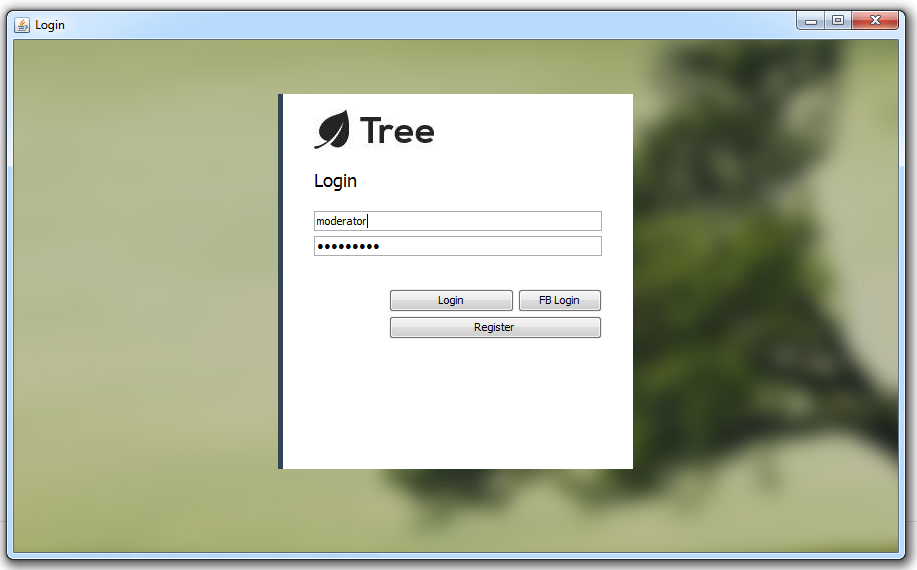
\includegraphics[width=12cm]{images/login.png}\\[.5cm]

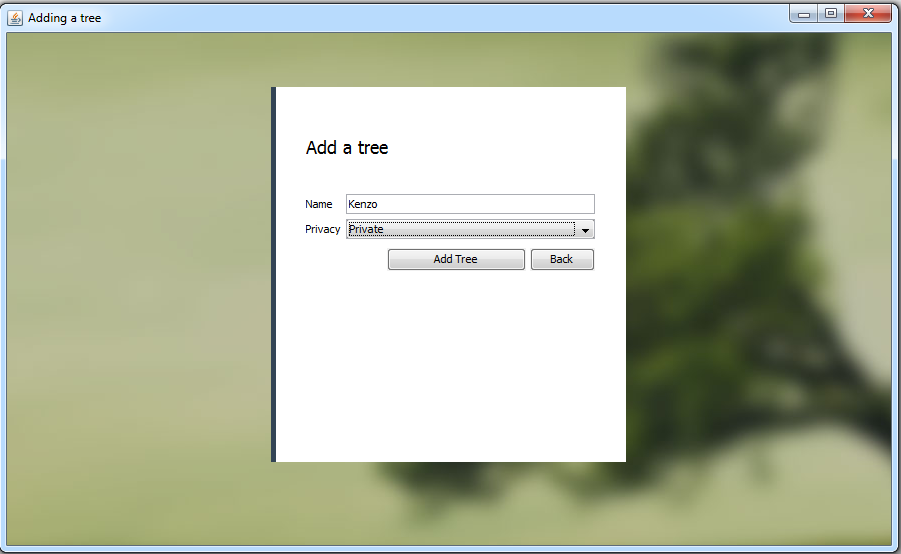
\includegraphics[width=12cm]{images/add_tree.png}\\[.5cm]
Er zijn 2 mogelijkheden om als gebruiker in te loggen.

\begin{enumerate}
\item \label{it:first}Inloggen door met gebruikersnaam en passwoord.



\item \label{it:first}Inloggen via facebook

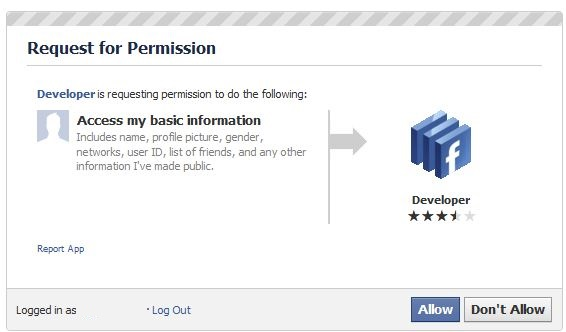
\includegraphics[width=12cm]{images/facebook.png}\\[.5cm]
\end{enumerate}

\subsection{Registratie}
Op het loginscherm kan je een gebruiker aanmaken door een naam en passwoord op te geven : 

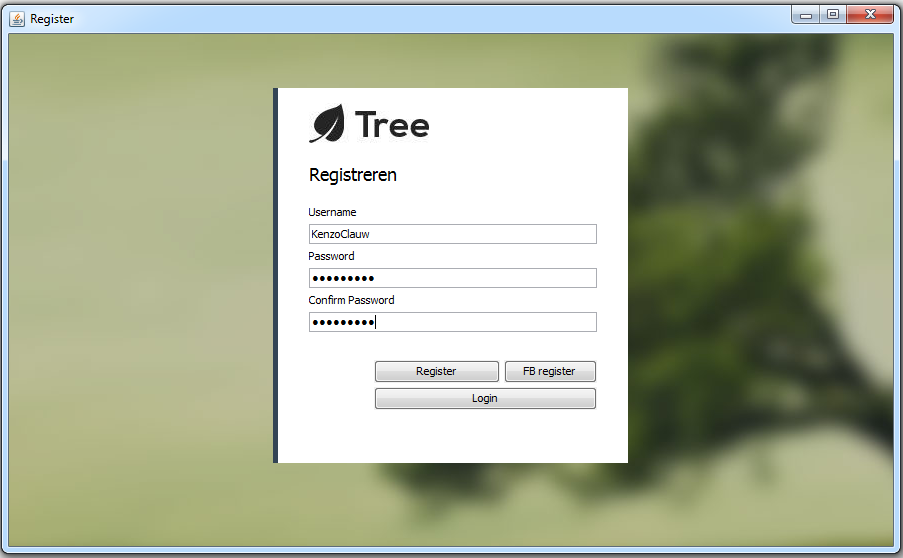
\includegraphics[width=12cm]{images/register.png}\\[.5cm]
Het passwoord moet minimum 8 characters lang zijn.
Na het registreren wordt je terug doorverwezen naar het login scherm.


\chapter{Overzicht stambomen}\label{ch:preface}
Na het inloggen als een gewone gebruiker krijg je een overzicht van stambomen.

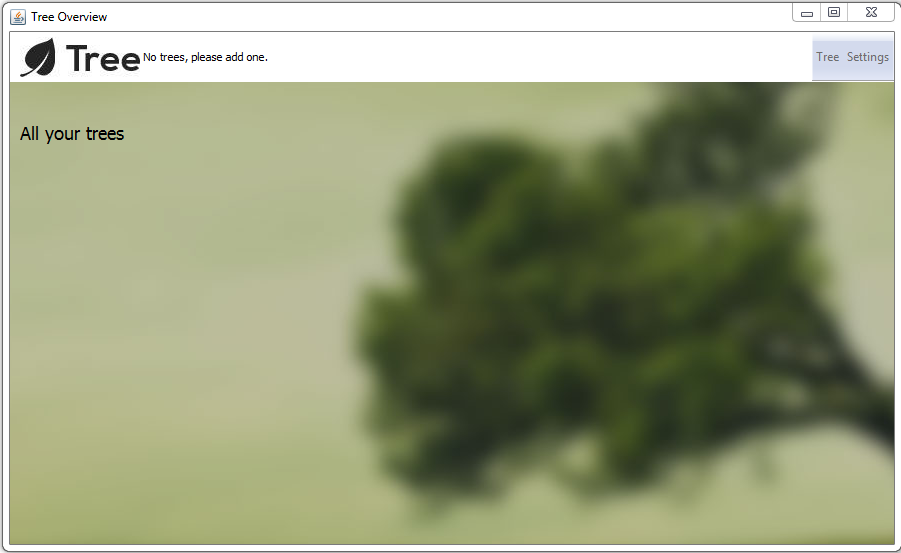
\includegraphics[width=12cm]{images/user_treeoverview.png}\\[.5cm]

Een stamboom toevoegen kan via het menu Tree.
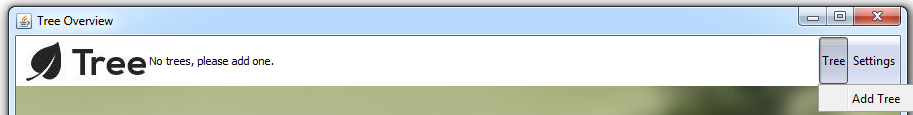
\includegraphics[width=12cm]{images/tree_add.png}\\[.5cm]

Er verschijnt een panel je een naam moet opgeven en 1 van de volgende privacy instellingen selecteren :

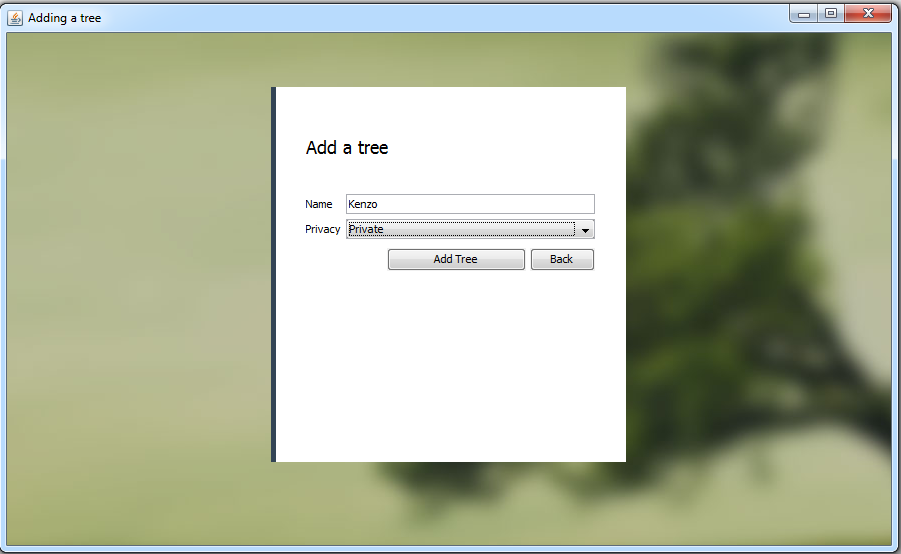
\includegraphics[width=12cm]{images/add_tree.png}\\[.5cm]

\begin{enumerate}
\item \label{it:first}Private
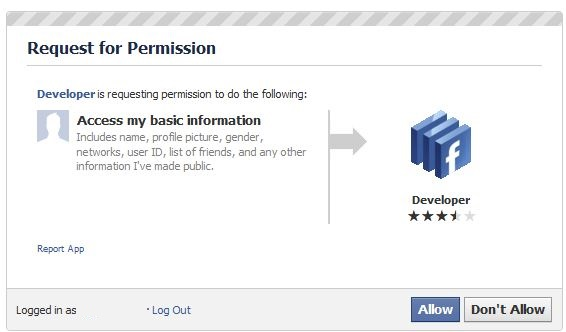
\includegraphics[width=12cm]{images/facebook.png}\\[.5cm]
\end{enumerate}

Na het toevoegen van een tree krijg je terug een overzicht van de stambomen.

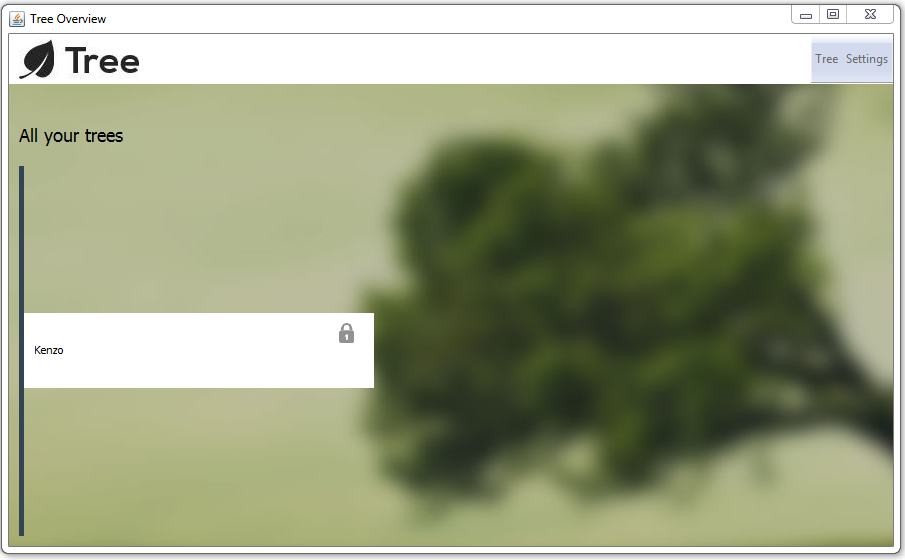
\includegraphics[width=12cm]{images/user_treeoverview_full.png}\\[.5cm]

\chapter{Settings}
\subsection{Taal}
Om de taal van de applicatie te wijzigen :
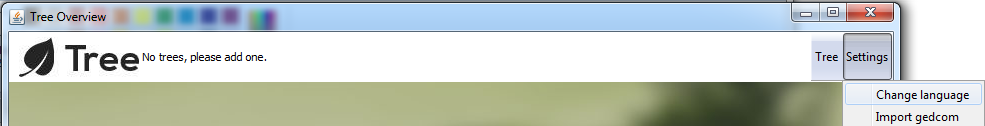
\includegraphics[width=12cm]{images/change_language.png}\\[.5cm]
\subsection{Gedcom}
Om een gedcom bestand te importeren :
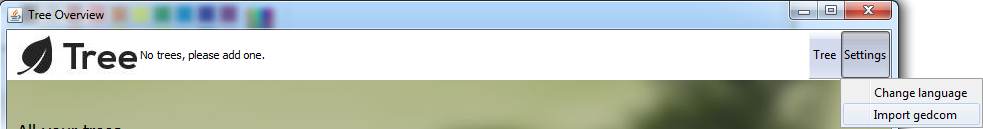
\includegraphics[width=12cm]{images/import_gedcom.png}\\[.5cm]


\chapter{Administrator}
%%%%%%%%%%%%%%%%%%%%%%%%%%%%%%%%%%%%%%%%%%%%%%%%%%%%%%%%%%%%%
%% APPENDICES
%%%%%%%%%%%%%%%%%%%%%%%%%%%%%%%%%%%%%%%%%%%%%%%%%%%%%%%%%%%%%

\appendix
%\input{FileName} %You need a file 'FileName.tex' for this.

\end{document}

